\subsection{Architecture logicielle des \emph{GUI}}
\label{sec:archi-log-gui}

\par Conscient du fonctionnement de la librairie graphique \emph{Swing}, nous avons décidé d'implémenter toutes nos IU avec le même schéma. Schéma que vous retrouvez à la figure \ref{fig:archi-log-gui}.

\begin{figure}[h!]
  \centering
  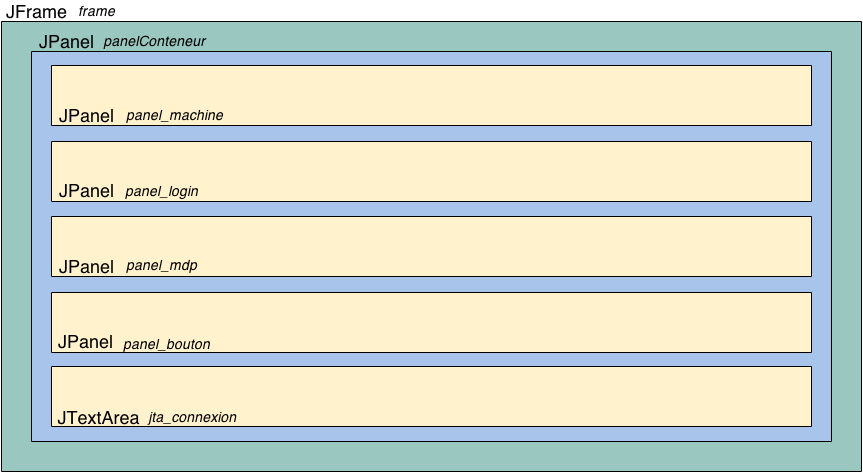
\includegraphics[width=11cm]{images/archi_log_iu.png}
  \caption{Architecture logicielle des \emph{GUI}}
  \label{fig:archi-log-gui}
\end{figure}

\par À chaque IU correspond un seul \emph{JFrame}. Dans celui-ci, un \emph{JPanel} appelé \emph{Content Pane}, contenu dans le \emph{frame}, englobe la totalité des \emph{JPanel} qui à leurs tour englobent les autres composants de la IU. Il y a donc une arborescence qui part de la fenêtre en elle-même (le \emph{frame}) jusqu’aux éléments qui la composant (\emph{JTextField}, \emph{JLabel}, \emph{JTextArea}, \emph{JButton}). La figure \vref{fig:archi-log-gui} donne la répartition des différents composants.

\begin{figure}[h!]
  \centering
  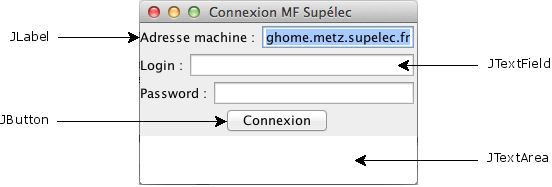
\includegraphics[width=11cm]{images/iuconnexion_launch_archi.png}
  \caption{IU de connexion : composants du \emph{JFrame}}
  \label{fig:archi-log-gui2}
\end{figure}

%%% Local Variables: 
%%% mode: latex
%%% TeX-master: "CompteRendu"
%%% End: 